\apendice{Especificación de Requisitos}

Si procede.


\section{Diagrama de casos de uso}

% Inicio de la figura
\begin{figure}[h]
    \centering
    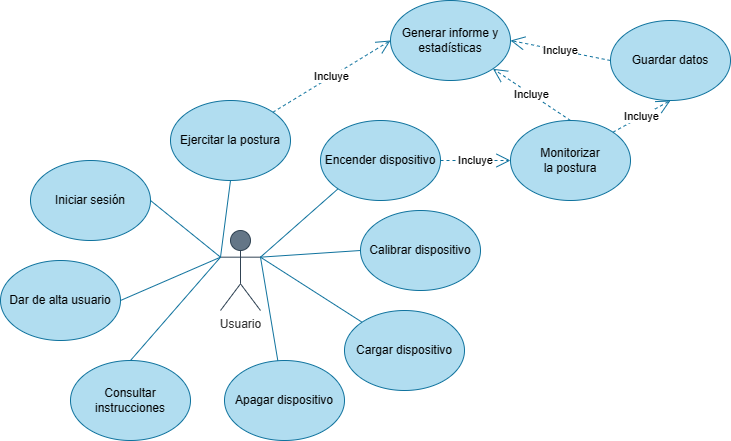
\includegraphics[width=1\textwidth]{img/DiagramaCasosDeUso.png}
    \caption{Diagrama de casos de uso}
    \label{fig:Casosuso} % Esta etiqueta es la que permite que se encuentr referenciada en el texto (es muy importante que siempre estén referenciadas en el texto)
\end{figure}

\section{Explicación casos de uso.}



Se puede describir mediante el uso de tablas o mediante lenguaje natural.   

Una muestra de cómo podría ser una tabla de casos de uso:

\begin{comment}
% Caso de Uso 1 -> Consultar Experimentos.
\begin{table}[p]
	\centering
	\begin{tabularx}{\linewidth}{ p{0.21\columnwidth} p{0.71\columnwidth} }
		%\toprule
		\multicolumn{1}{|l|} {\cellcolor[HTML]{68CBD0}\textbf{CU-1}}    & \multicolumn{1}{l|}{\textbf{Ejemplo de caso de uso}}\\
		%\toprule
		\textbf{Versión}              & 1.0    \\
		\textbf{Autor}                & Alumno \\
		\textbf{Requisitos asociados} & RF-xx, RF-xx \\
		\textbf{Descripción}          & La descripción del CU \\
		\textbf{Precondición}         & Precondiciones (podría haber más de una) \\
		\textbf{Acciones}             &
		\begin{enumerate}
			\def\labelenumi{\arabic{enumi}.}
			\tightlist
			\item Pasos del CU
			\item Pasos del CU (añadir tantos como sean necesarios)
		\end{enumerate}\\
		\textbf{Postcondición}        & Postcondiciones (podría haber más de una) \\
		\textbf{Excepciones}          & Excepciones \\
		\textbf{Importancia}          & Alta o Media o Baja... \\
		\bottomrule
	\end{tabularx}
	\caption{CU-1 Nombre del caso de uso.}
\end{table}
\end{comment}


% Comentamos las tablas de ejemplo
\begin{comment}
% Caso de Uso 2 -> Consultar Experimentos.
\begin{table}[p]
	\centering
        
	\begin{tabularx}{\linewidth}{ p{0.21\columnwidth} p{0.71\columnwidth} }
		%\toprule
        \hline
		\multicolumn{3}{|c|} {\cellcolor[HTML]{68CBD0}\textbf{CU-1}}    & \multicolumn{1}{|c|}{\textbf{Ejemplo de caso de uso}}\\
		%\toprule
  \hline
		\multicolumn{1}{|l|}{\textbf{Versión}}              & 1.0    \\
		\textbf{Autor}                & Alumno \\
		\textbf{Requisitos asociados} & RF-xx, RF-xx \\
		\textbf{Descripción}          & La descripción del CU \\
		\textbf{Precondición}         & Precondiciones (podría haber más de una) \\
		\textbf{Acciones}             &
		\begin{enumerate}
			\def\labelenumi{\arabic{enumi}.}
			\tightlist
			\item Pasos del CU
			\item Pasos del CU (añadir tantos como sean necesarios)
		\end{enumerate}\\
		\textbf{Postcondición}        & Postcondiciones (podría haber más de una) \\
		\textbf{Excepciones}          & Excepciones \\
		\textbf{Importancia}          & Alta o Media o Baja... \\
		\bottomrule
	\end{tabularx}
	\caption{CU-2 Nombre del caso de uso.}
\end{table}
\end{comment}

% ----------------------------------------------------
% ----------------------------------------------------
% Caso de uso 01
\begin{table}[h!]
\centering
\begin{tabular}{ |m{3cm}|m{11cm}|  } 
\hline
\cellcolor[HTML]{B9E3F0}\centering\textbf{CS-01} & \cellcolor[HTML]{B9E3F0}\textbf{<Encender dispositivo>}\\

\hline
\cellcolor[HTML]{EFEFEF}\textbf{Versión}             & 1.0  \\
\hline
\cellcolor[HTML]{EFEFEF}\textbf{Autor}                & Naiara Gadea Rodíguez Gómez\\
\hline
\cellcolor[HTML]{EFEFEF}\textbf{Descripción}                & {Puesta en marcha del dispositivo hardware y su conexión con la aplicación. El dispositivo no deberá estar siempre conectado con la aplicación, pero si se conecta a la aplicación se puede obtener más información. }\\
\hline
\cellcolor[HTML]{EFEFEF}\textbf{Secuencia \newline Normal}                &                 
        \begin{enumerate}
			\def\labelenumi{\arabic{enumi}.}
			\tightlist
			\item Se coloca el dispositivo en contacto sobre la piel, como se indica en las instrucciones.
			\item Se enciende el dispositivo con el botón ON/OFF.
                \item Cuando se encienda un led verde indicará que el dispositivo está encendido.  
                \item Se conecta el dispositivo al dispositivo que tiene instalada la aplicación vía Bluetooth o vía WIFI.
                \item El usuario accede a la aplicación software instalada en el dispositivo móvil o en el ordenador, que deberán estar conectados a la misma red WIFI o Bluetooth para permitir la comunicación.  
                \item Una vez se realiza la conexión, el led verde del dispositivo cambia a color a azul. Además, en la aplicación aparece el dispositivo como conectado. 
		\end{enumerate}\\
\hline
\cellcolor[HTML]{EFEFEF}\textbf{Frecuencia}                & Alta\\
\hline
\cellcolor[HTML]{EFEFEF}\textbf{Importancia}                & Alta\\
\hline
\cellcolor[HTML]{EFEFEF}\textbf{Urgencia}                & Alta\\
\hline
\cellcolor[HTML]{EFEFEF}\textbf{Requisitos Funcionales Relacionados}                & {RF-02}\\
\hline
\cellcolor[HTML]{EFEFEF}\textbf{Casos de uso relacionados}                & {CS-02, CS-03, CS-04, CS-07, CS-08, CS-10}\\
\hline
\end{tabular}
\caption{CU-01. Encender dispositivo.}
\end{table}

% ----------------------------------------------------
% Caso de uso 02
\begin{table}[h!]
\centering
\begin{tabular}{ |m{3cm}|m{11cm}|  } 
\hline
\cellcolor[HTML]{B9E3F0}\textbf{CS-02} & \cellcolor[HTML]{B9E3F0}\textbf{<Apagar dispositivo>}\\

\hline
\cellcolor[HTML]{EFEFEF}\textbf{Versión}             & 1.0  \\
\hline
\cellcolor[HTML]{EFEFEF}\textbf{Autor}                & Naiara Gadea Rodíguez Gómez\\
\hline
\cellcolor[HTML]{EFEFEF}\textbf{Descripción}                & {Apagado del dispositivo.}\\
\hline
\cellcolor[HTML]{EFEFEF}\textbf{Secuencia \newline Normal}                &                 
        \begin{enumerate}
			\def\labelenumi{\arabic{enumi}.}
			\tightlist
			\item Se apaga el dispositivo con el botón ON/OFF.
			\item Una vez el dispositivo se encuentre apagado el led azul o verde se apagará.
                \item El usuario se puede quitar el dispositivo y puede cargarlo.
		\end{enumerate}\\
\hline
\cellcolor[HTML]{EFEFEF}\textbf{Frecuencia}                & Alta\\
\hline
\cellcolor[HTML]{EFEFEF}\textbf{Importancia}                & Alta\\
\hline
\cellcolor[HTML]{EFEFEF}\textbf{Urgencia}                & Media\\
\hline
\cellcolor[HTML]{EFEFEF}\textbf{Requisitos Funcionales Relacionados}                & {RF-02}\\
\hline
\cellcolor[HTML]{EFEFEF}\textbf{Casos de uso relacionados}                & {CS-01, CS-03}\\
\hline
\cellcolor[HTML]{EFEFEF}\textbf{Comentarios}                & {El dispositivo también se apaga cuando se acaba la batería, en cuyo caso el caso de uso comienza en el paso 2. }\\
\hline
\end{tabular}
\caption{CU-02. Apagar dispositivo.}
\end{table}

% ----------------------------------------------------
% Caso de uso 03
\begin{table}[h!]%[p]
\centering
\begin{tabular}{ |m{3cm}|m{11cm}|  } 
\hline
\cellcolor[HTML]{B9E3F0}\textbf{CS-03} & \cellcolor[HTML]{B9E3F0}\textbf{<Cargar dispositivo>}\\

\hline
\cellcolor[HTML]{EFEFEF}\textbf{Versión}             & 1.0  \\
\hline
\cellcolor[HTML]{EFEFEF}\textbf{Autor}                & Naiara Gadea Rodíguez Gómez\\
\hline
\cellcolor[HTML]{EFEFEF}\textbf{Descripción}                & {Carga de la batería del dispositivo empleando la estación de carga.}\\
\hline
\cellcolor[HTML]{EFEFEF}\textbf{Secuencia \newline Normal}                &                 
        \begin{enumerate}
			\def\labelenumi{\arabic{enumi}.}
			\tightlist
			\item Actúa el CS-02. 
			\item Una vez que el dispositivo se encuentre apagado el usuario coloca el dispositivo sobre la estación de carga enchufada a la corriente.
                \item Se enciende un led rojo intermitente.
                \item Cuando la batería del dispositivo se encuentre completamente cargada, el led rojo intermitente deja de ser intermitente.
                \item El dispositivo está completamente cargado y puede desconectar la estación de carga de la corriente o desconectar el dispositivo.
                \item El dispositivo estará listo para su uso.
		\end{enumerate}\\
\hline
\cellcolor[HTML]{EFEFEF}\textbf{Frecuencia}                & Alta\\
\hline
\cellcolor[HTML]{EFEFEF}\textbf{Importancia}                & Alta\\
\hline
\cellcolor[HTML]{EFEFEF}\textbf{Urgencia}                & Media\\
\hline
\cellcolor[HTML]{EFEFEF}\textbf{Requisitos Funcionales Relacionados}                & {RF-08}\\
\hline
\cellcolor[HTML]{EFEFEF}\textbf{Casos de uso relacionados}                & {CS-02}\\
\hline
\end{tabular}
\caption{CU-03. Cargar dispositivo.}
\end{table}

% ----------------------------------------------------
% Caso de uso 04
\begin{table}[h!]
\centering
\begin{tabular}{ |m{3cm}|m{11cm}|  } 
\hline
\cellcolor[HTML]{B9E3F0}\textbf{CS-04} & \cellcolor[HTML]{B9E3F0}\textbf{<Calibrar dispositivo>}\\

\hline
\cellcolor[HTML]{EFEFEF}\textbf{Versión}             & 1.0  \\
\hline
\cellcolor[HTML]{EFEFEF}\textbf{Autor}                & Naiara Gadea Rodíguez Gómez\\
\hline
\cellcolor[HTML]{EFEFEF}\textbf{Descripción}                & {Se recalculan los valores en reposo para que el dispositivo devuelva medidas lo más precisas posible. Se debe calibrar el dispositivo cada cierto tiempo para que los valores medidos sean lo más precisos posible.}\\
\hline
\cellcolor[HTML]{EFEFEF}\textbf{Secuencia \newline Normal}                &                 
        \begin{enumerate}
			\def\labelenumi{\arabic{enumi}.}
			\tightlist
			\item El dispositivo debe estar encendido y sobre una superficie plana.
			\item Se presionará el botón de calibrado. Sobre el dispositivo o de la propia aplicación. 
                \item El sistema recalibra los valores medidos por el dispositivo.
                \item Una vez el dispositivo se haya calibrado correctamente se encenderá 3 veces el led verde o azul, en función si la calibración se ha realizado a través de la aplicación o directamente sobre el dispositivo. 
                \item El dispositivo se encuentra correctamente calibrado y listo para su uso. 
		\end{enumerate}\\
\hline
\cellcolor[HTML]{EFEFEF}\textbf{Frecuencia}                & Baja\\
\hline
\cellcolor[HTML]{EFEFEF}\textbf{Importancia}                & Alta\\
\hline
\cellcolor[HTML]{EFEFEF}\textbf{Urgencia}                & Baja\\
\hline
\cellcolor[HTML]{EFEFEF}\textbf{Requisitos Funcionales Relacionados}                & {RF-01, RF-04}\\
\hline
\cellcolor[HTML]{EFEFEF}\textbf{Casos de uso relacionados}                & {CS-01, CS-07}\\
\hline
\end{tabular}
\caption{CU-04. Calibrar dispositivo.}
\end{table}

% ----------------------------------------------------
% Caso de uso 05
\begin{table}[h!]
\centering
\begin{tabular}{ |m{3cm}|m{11cm}|  } 
\hline
\cellcolor[HTML]{B9E3F0}\textbf{CS-05} & \cellcolor[HTML]{B9E3F0}\textbf{<Dar de alta usuario>}\\

\hline
\cellcolor[HTML]{EFEFEF}\textbf{Versión}             & 1.0  \\
\hline
\cellcolor[HTML]{EFEFEF}\textbf{Autor}                & Naiara Gadea Rodíguez Gómez\\
\hline
\cellcolor[HTML]{EFEFEF}\textbf{Descripción}                & {El usuario crea una cuenta para cada recopilar los datos recopilados por el dispositivo. Se creará una cuenta por persona que vaya a utilizar el dispositivo.}\\
\hline
\cellcolor[HTML]{EFEFEF}\textbf{Secuencia \newline Normal}                &                 
        \begin{enumerate}
			\def\labelenumi{\arabic{enumi}.}
			\tightlist
			\item El caso de uso comienza cuando el facultativo clica en registrar.
			\item El sistema solicita el nombre de usuario. 
                \item El usuario introduce el nombre de usuario.
                \item El sistema solicita los nombre y apellidos del usuario.
                \item El usuario introduce su nombre y apellidos.
                \item El sistema solicita una contraseña. 
                \item El usuario introduce una contraseña. 
                \item El sistema guarda y almacena los datos introducidos. Se ha creado la cuenta del usuario. 
		\end{enumerate}\\
\hline
\cellcolor[HTML]{EFEFEF}\textbf{Frecuencia}                & Baja\\
\hline
\cellcolor[HTML]{EFEFEF}\textbf{Importancia}                & Media\\
\hline
\cellcolor[HTML]{EFEFEF}\textbf{Urgencia}                & Media\\
\hline
\cellcolor[HTML]{EFEFEF}\textbf{Requisitos Funcionales Relacionados}                & {RF-01, RF-03 }\\
\hline
\cellcolor[HTML]{EFEFEF}\textbf{Casos de uso relacionados}                & {CS-06}\\
\hline
\end{tabular}
\caption{CU-05. Dar de alta usuario.}
\end{table}

% ----------------------------------------------------
% Caso de uso 06
\begin{table}[h!]
\centering
\begin{tabular}{ |m{3cm}|m{11cm}|  } 
\hline
\cellcolor[HTML]{B9E3F0}\textbf{CS-06} & \cellcolor[HTML]{B9E3F0}\textbf{<Iniciar sesión>}\\

\hline
\cellcolor[HTML]{EFEFEF}\textbf{Versión}             & 1.0  \\
\hline
\cellcolor[HTML]{EFEFEF}\textbf{Autor}                & Naiara Gadea Rodíguez Gómez\\
\hline
\cellcolor[HTML]{EFEFEF}\textbf{Descripción}                & {El usuario inicia sesión en la aplicación para poder acceder a sus datos, informes y ejercicios. El usuario tiene la opción de mantener la sesión iniciada. }\\
\hline
\cellcolor[HTML]{EFEFEF}\textbf{Secuencia \newline Normal}                &                 
        \begin{enumerate}
			\def\labelenumi{\arabic{enumi}.}
			\tightlist
			\item El sistema solicita nombre de usuario y contraseña.
			\item El usuario introduce su nombre de usuario y contraseña. 
                \item El sistema pregunta si desea mantener la sesión abierta.
                \item El usuario introduce si desea mantener la sesión abierta. 
                \item El sistema compara con su base de datos y si encuentra coincidencia accede a los datos del usuario. En caso de que no encuentre al usuario el sistema imprime por pantalla ‘Contraseña o usuario incorrectos’.
                \item El sistema muestra las estadísticas y datos del paciente.
		\end{enumerate}\\
\hline
\cellcolor[HTML]{EFEFEF}\textbf{Frecuencia}                & Media\\
\hline
\cellcolor[HTML]{EFEFEF}\textbf{Importancia}                & Alta\\
\hline
\cellcolor[HTML]{EFEFEF}\textbf{Urgencia}                & Media\\
\hline
\cellcolor[HTML]{EFEFEF}\textbf{Requisitos Funcionales Relacionados}                & {RF-01, RF-03, RF-06 }\\
\hline
\cellcolor[HTML]{EFEFEF}\textbf{Casos de uso relacionados}                & {CS-05, CS-07, CS-08, CS-09, CS-10}\\
\hline
\cellcolor[HTML]{EFEFEF}\textbf{Comentarios}                & {Si el usuario ha indicado que desea mantener la sesión abierta, la sesión se mantiene abierta, aunque se cierre la aplicación. El usuario deberá cerrar manualmente su sesión. }\\
\hline
\end{tabular}
\caption{CU-06. Iniciar sesión.}
\end{table}

% ----------------------------------------------------
% Caso de uso 07
\begin{table}[h!]
\centering
\begin{tabular}{ |m{3cm}|m{11cm}|  } 
\hline
\cellcolor[HTML]{B9E3F0}\textbf{CS-07} & \cellcolor[HTML]{B9E3F0}\textbf{<Realizar monitoreo de la postura>}\\

\hline
\cellcolor[HTML]{EFEFEF}\textbf{Versión}             & 1.0  \\
\hline
\cellcolor[HTML]{EFEFEF}\textbf{Autor}                & Naiara Gadea Rodíguez Gómez\\
\hline
\cellcolor[HTML]{EFEFEF}\textbf{Descripción}                & {Una vez el dispositivo se encuentre encendido se realiza la monitorización de la postura. Si se detecta una mala postura el dispositivo emitirá una vibración. En el caso de que el dispositivo se encuentre conectado con la aplicación los datos.}\\
\hline
\cellcolor[HTML]{EFEFEF}\textbf{Secuencia \newline Normal}                &                 
        \begin{enumerate}
			\def\labelenumi{\arabic{enumi}.}
			\tightlist
			\item El caso de uso comienza cuando se enciende el usuario enciende el dispositivo. 
			\item Pasos del CU El sistema obtiene los datos proporcionados por el sensor del dispositivo. 
                \item El sistema identifica entre una buena o mala postura, gracias al algoritmo. 
                \item Si se detecta mala postura el dispositivo emita una señal vibratoria para que el usuario modifique su postura.
                \item Interviene el CS-08. 
                \item El caso de uso finaliza cuando se apaga el dispositivo o cuando se gasta la batería del dispositivo.
		\end{enumerate}\\
\hline
\cellcolor[HTML]{EFEFEF}\textbf{Frecuencia}                & Alta\\
\hline
\cellcolor[HTML]{EFEFEF}\textbf{Importancia}                & Alta\\
\hline
\cellcolor[HTML]{EFEFEF}\textbf{Urgencia}                & Alta\\
\hline
\cellcolor[HTML]{EFEFEF}\textbf{Requisitos Funcionales Relacionados}                & {RF-02, RF-04, RF-05 }\\
\hline
\cellcolor[HTML]{EFEFEF}\textbf{Casos de uso relacionados}                & {CS- 01, CS-04, CS-06, CS-08, CS-09, CS-10 }\\
\hline
\end{tabular}
\caption{CU-07. Realizar monitoreo de la postura.}
\end{table}

% ----------------------------------------------------
% Caso de uso 08
\begin{table}[h!]
\centering
\begin{tabular}{ |m{3cm}|m{11cm}|  } 
\hline
\cellcolor[HTML]{B9E3F0}\textbf{CS-08} & \cellcolor[HTML]{B9E3F0}\textbf{<Guardar datos>}\\

\hline
\cellcolor[HTML]{EFEFEF}\textbf{Versión}             & 1.0  \\
\hline
\cellcolor[HTML]{EFEFEF}\textbf{Autor}                & Naiara Gadea Rodíguez Gómez\\
\hline
\cellcolor[HTML]{EFEFEF}\textbf{Descripción}                & {Se archivan los datos recopilados a través del dispositivo. Los datos se van guardando en tiempo real si el dispositivo se encuentra conectado a la aplicación.}\\
\hline
\cellcolor[HTML]{EFEFEF}\textbf{Secuencia \newline Normal}                &                 
        \begin{enumerate}
			\def\labelenumi{\arabic{enumi}.}
			\tightlist
			\item El sistema registra los datos enviados vía Bluetooth o WIFI por el dispositivo.
			\item Interviene el CS-07.
                \item El sistema guarda los datos y el informe generado en la base de datos integrada. Que se podrán consultar posteriormente o en tiempo real.
		\end{enumerate}\\
\hline
\cellcolor[HTML]{EFEFEF}\textbf{Frecuencia}                & Alta\\
\hline
\cellcolor[HTML]{EFEFEF}\textbf{Importancia}                & Alta\\
\hline
\cellcolor[HTML]{EFEFEF}\textbf{Urgencia}                & Alta\\
\hline
\cellcolor[HTML]{EFEFEF}\textbf{Requisitos Funcionales Relacionados}                & {RF-01, RF-02, RF-04, RF-06} \\
\hline
\cellcolor[HTML]{EFEFEF}\textbf{Casos de uso relacionados}                & {CS-06, CS-07, CS-09}\\
\hline
\end{tabular}
\caption{CU-08. Guardar datos.}
\end{table}

% ----------------------------------------------------
% Caso de uso 09
\begin{table}[h!]
\centering
\begin{tabular}{ |m{3cm}|m{11cm}|  } 
\hline
\cellcolor[HTML]{B9E3F0}\textbf{CS-09} & \cellcolor[HTML]{B9E3F0}\textbf{<Generar informe>}\\

\hline
\cellcolor[HTML]{EFEFEF}\textbf{Versión}             & 1.0  \\
\hline
\cellcolor[HTML]{EFEFEF}\textbf{Autor}                & Naiara Gadea Rodíguez Gómez\\
\hline
\cellcolor[HTML]{EFEFEF}\textbf{Descripción}                & {A partir de los datos recopilados del sensor, se realiza un informe que puede ser en tiempo real que incluye toda la información relevante y estadísticas calculadas en función de los datos. }\\
\hline
\cellcolor[HTML]{EFEFEF}\textbf{Secuencia \newline Normal}                &                 
        \begin{enumerate}
			\def\labelenumi{\arabic{enumi}.}
			\tightlist
			\item El caso de uso comienza tras el CS-08.
			\item El sistema incluye los datos obtenidos. 
                \item El sistema crea varias estadísticas utilizando gráficas que resumen visualmente los datos recogidos y la evolución del paciente.
                \item Se puede obtener un informe en formato pdf. 
		\end{enumerate}\\
\hline
\cellcolor[HTML]{EFEFEF}\textbf{Frecuencia}                & Alta\\
\hline
\cellcolor[HTML]{EFEFEF}\textbf{Importancia}                & Alta\\
\hline
\cellcolor[HTML]{EFEFEF}\textbf{Urgencia}                & Alta\\
\hline
\cellcolor[HTML]{EFEFEF}\textbf{Requisitos Funcionales Relacionados}                & {RF-01, RF-02, RF-04, RF-06 }\\
\hline
\cellcolor[HTML]{EFEFEF}\textbf{Casos de uso relacionados}                & {CS-06, CS-07, CS-08, CS-10 }\\
\hline
\end{tabular}
\caption{CU-09. Generar informe.}
\end{table}

% ----------------------------------------------------
% Caso de uso 10
\begin{table}[h!]
\centering
\begin{tabular}{ |m{3cm}|m{11cm}|  } 
\hline
\cellcolor[HTML]{B9E3F0}\textbf{CS-10} & \cellcolor[HTML]{B9E3F0}\textbf{<Ejercitar la musculatura de la postura>}\\

\hline
\cellcolor[HTML]{EFEFEF}\textbf{Versión}             & 1.0  \\
\hline
\cellcolor[HTML]{EFEFEF}\textbf{Autor}                & Naiara Gadea Rodíguez Gómez\\
\hline
\cellcolor[HTML]{EFEFEF}\textbf{Descripción}                & {Se realizan distintos juegos o ejercicios incluidos en la aplicación software, que, mediante la interacción con el dispositivo hardware, permitirán al usuario aumentar y mejorar la musculatura que se necesita para una buena postura. }\\
\hline
\cellcolor[HTML]{EFEFEF}\textbf{Secuencia \newline Normal}                &                 
        \begin{enumerate}
			\def\labelenumi{\arabic{enumi}.}
			\tightlist
			\item El usuario selecciona dentro de la pestaña de juegos y ejercicios, el juego o el ejercicio que desee realizar. 
			\item El sistema muestra el juego o ejercicio seleccionado. 
                \item El usuario realiza el juego o ejercicio seleccionado. 
                \item Una vez finalizado el juego o el ejercicio el sistema vuelve a la pantalla donde se incluyen los ejercicios y juegos disponibles para mejorar la musculatura o la postura. 
		\end{enumerate}\\
\hline
\cellcolor[HTML]{EFEFEF}\textbf{Frecuencia}                & Media\\
\hline
\cellcolor[HTML]{EFEFEF}\textbf{Importancia}                & Baja\\
\hline
\cellcolor[HTML]{EFEFEF}\textbf{Urgencia}                & Baja\\
\hline
\cellcolor[HTML]{EFEFEF}\textbf{Requisitos Funcionales Relacionados}                & {RF-01, RF-02, RF-04, RF-05 }\\
\hline
\cellcolor[HTML]{EFEFEF}\textbf{Casos de uso relacionados}                & {CS-01, CS-04, CS-06, CS-07, CS-09, CS-11}\\
\hline
\end{tabular}
\caption{CU-10. Ejercitar la musculatura de la postura.}
\end{table}

% ----------------------------------------------------
% Caso de uso 11
\begin{table}[h!]
\centering
\begin{tabular}{ |m{3cm}|m{11cm}|  } 
\hline
\cellcolor[HTML]{B9E3F0}\textbf{CS-11} & \cellcolor[HTML]{B9E3F0}\textbf{<Consultar instrucciones de uso>}\\

\hline
\cellcolor[HTML]{EFEFEF}\textbf{Versión}             & 1.0  \\
\hline
\cellcolor[HTML]{EFEFEF}\textbf{Autor}                & Naiara Gadea Rodíguez Gómez\\
\hline
\cellcolor[HTML]{EFEFEF}\textbf{Descripción}                & {El usuario puede revisar las instrucciones de uso del dispositivo, y de esa forma puede obtener información para la puesta en marcha para poder monitorizar su postura.}\\
\hline
\cellcolor[HTML]{EFEFEF}\textbf{Secuencia \newline Normal}                &                 
        \begin{enumerate}
			\def\labelenumi{\arabic{enumi}.}
			\tightlist
			\item El usuario clica sobre el icono ‘?’ donde se puede consultar las instrucciones.
			\item El sistema abre una pestaña con las instrucciones de uso que puede seguir el usuario. Las instrucciones serán sencillas y deberán redirigir a un vídeo explicativo de la puesta en marcha y uso del dispositivo.
                \item El usuario cierra la ventana de instrucciones cuando deje de necesitar su consulta. 
		\end{enumerate}\\
\hline
\cellcolor[HTML]{EFEFEF}\textbf{Frecuencia}                & Baja\\
\hline
\cellcolor[HTML]{EFEFEF}\textbf{Importancia}                & Baja\\
\hline
\cellcolor[HTML]{EFEFEF}\textbf{Urgencia}                & Baja\\
\hline
\cellcolor[HTML]{EFEFEF}\textbf{Requisitos Funcionales Relacionados}                & {RF-02, RF-07}\\
\hline
\cellcolor[HTML]{EFEFEF}\textbf{Casos de uso relacionados}                & {CS-01, CS-02, CS-03, CS-04, CS-05, CS-06, CS-07, CS-09, CS-10 }\\
\hline
\end{tabular}
\caption{CU-11. Consultar instrucciones de uso.}
\end{table}


%%%%%%%%%%%%%%%%%%%%%%%%%%%%%%%%%%%%%%
\clearpage

\section{Prototipos de interfaz o interacción con el proyecto.}
